\section{Математическая модель эффекта обратной связи}
\label{sec:mainres}
    \subsection{Предварительные и вспомогательные результаты}
    \paragraph{Обозначения.}
        Множество $\textbf{F}$ функций плотности вероятности, определяется как

        \begin{equation} \label{R}
            \textbf{F} := \left\{f : \mathbb{R}^n \rightarrow \mathbb{R}_+ ~\text{и}~ \int_{\mathbb{R}^n}f(x)dx = 1\right\}.
        \end{equation}
        
        Пусть $f(x), x \in \mathbb{R}^n$, -- функция плотности вероятности из $\textbf{F}$, $g(x)$ -- измеримая по Лебегу функция из $L_1(\mathbb{R}^n)$, а $\{\psi_t\}_{t = 0}^{\infty} > 0$ -- неотрицательная последовательность из $\mathbb{R}$. 

        Применения последовательности из $t$ отображений $\{\text{D}_t\}$ удобно обозначить через $\text{D}_{\overline{1, t}}(\cdot) := \text{D}_t(\text{D}_{t-1} ( ... \text{D}_1( \cdot ) ... ))$.

        Пусть $\phi(x)$ -- любая непрерывная функция с компактным носителем. В данной работе используется дельта-функция Дирака $\delta(x)$, определяемая как 
        $
           \int_{\mathbb{R}^n} \delta(x) \phi(x) dx =  \phi(0) ~ \forall \phi(x)
        $, и \emph{нулевое распределение} $\zeta(x)$, которое определяется как
        $
        \int_{\mathbb{R}^n} \zeta(x) \phi(x) dx =  0 ~ \forall \phi(x).
        $

        Будем говорить, что $f_t(x) \underset{t \to +\infty}{\longrightarrow} f(x)$ \emph{слабо}, когда 
        $
            \int_{\mathbb{R}^n} f_t(x) \phi(x) \, dx \underset{t \to +\infty}{\longrightarrow} \int_{\mathbb{R}^n} f(x) \phi(x) dx ~~ \forall \phi(x).
        $

        Также в работе используется классическое определение $k$-того момента случайной величины, определяемое как 
        $
        \nu_{k} := \mathbb{E}[\xi^k] = \int_{\mathbb{R}} x^{k} f_{\xi}(x) dx,
        $
        где $f_{\xi}(x)$ -- функция плотности случайной величины $\xi$.

        Теперь определим полезные свойства исследуемой задачи. Сначала рассмотрим случай, когда система не обязательно автономна, то есть имеет вид \eqref{system}.

        \begin{theorem}[По \cite{feller1991introduction}] \label{based}
            Если функция $f: \mathbb{R}^n \to \mathbb{R}$ такая, что $f(x) \geq 0$ для почти всех $x \in \mathbb{R}^n$ и $\|f\|_1 = \int\limits_{\mathbb{R}^n} f(x) dx = 1$, тогда существует случайный вектор $\mathbf{\xi}$, для которого $f$ будет его функцией плотности распределения.
        \end{theorem}

        Именно на основе Теоремы~\ref{based} множество $\textbf{F}$ определено таким образом \eqref{R}. Хотя на практике наблюдаются только отдельные выборки из данных на каждом шаге $t$, Теорема~\ref{based} связывает эти выборки со случайным вектором и его функцией плотности распределения. Для того, чтобы модель динамической системы \eqref{system} была интерпретируемой и практически применимой, нам нужно, чтобы каждая функция $f \in \textbf{F}$ была плотностью вероятности какого-то случайного вектора. 

        Теперь выведем условия, при которых произвольное отображение $\text{D}_t$ является преобразованием на $\textbf{F}$, то есть $\text{D}_t$ переводит $\textbf{F}$ в $\textbf{F}$.

        \begin{theorem}[Теорема 2 из \cite{veprikov2024mathematical}] \label{R_to_R}
            Если $\| \cdot \|_1$ норма отображения $\text{D}_t$ равняется единице: $\| \text{D}_t \|_1 = 1$, и для всех функций плотности $f(x) \in \textbf{F}$ выполнено $\text{D}_t(f)(x) \geq 0$ для почти всех $x \in \mathbb{R}^n$, и существует обратное отображение $\text{D}_t^{-1}$, такое что $\|\text{D}_t^{-1}\|_1 \leq 1$, тогда $\text{D}_t$ является преобразованием на $\textbf{F}$.
        \end{theorem}
        \begin{proof}
             Для начала заметим, что если $\text{D}_t: \textbf{F} \to \textbf{F}$, то $\|\text{D}_t\|_1 = 1$, потому что по определению нормы отображения:
            $
                \|\text{D}_t\|_1 = \sup_{\|f\|_1 = 1}\left\{\|\text{D}_t(f)\|_1\right\}.
            $
            И если $f$ такая, что $\|f\|_1 = 1$, то $|f| \in \textbf{F}$ и, так как $\text{D}_t: \textbf{F} \to \textbf{F}$, $\|\text{D}_t(|f|)\|_1 = 1$. Однако $\|\text{D}_t\|_1 = 1$ только необходимое, но не достаточное условие.
    
            Если $\|\text{D}_t\|_1 = 1$, тогда для всех $f \in \textbf{F}$ выполнено $\|\text{D}_t(f)\|_1 \leq 1$. Если существует $f_0 \in \textbf{F}$ такая, что $\|\text{D}_t(f_0)\|_1 < 1$, тогда получаем противоречие, так как
            \begin{multline*}
                \|D^{-1}\|_1 \overset{def}{=} \underset{\|f\|_1 \neq 0}{\sup}\left\{\dfrac{\|\text{D}_t^{-1}(f)\|_1}{\|f\|_1}\right\} 
                \geq \left[f_1 = \text{D}_t(f_0)\right] \geq
                \dfrac{\|\text{D}_t^{-1}(f_1)\|_1}{\|f_1\|_1} = \\ = 
                \dfrac{\|\text{D}_t^{-1}(\text{D}_t(f_0))\|_1}{\|\text{D}_t(f_0)\|_1} = 
                \dfrac{\|f_0\|_1}{\|\text{D}_t(f_0)\|_1} = \dfrac{1}{\|\text{D}_t(f_0)\|_1} > 1.
            \end{multline*}

            Если предположить, что $\|\text{D}_t^{-1}\|_1 \leq 1$, тогда для всех $f \in \textbf{F}$ выполнено $\|\text{D}_t(f)\|_1 = 1$.
    
            Согласно Теореме~\ref{based} для того, чтобы $\text{D}_t : \textbf{F} \to \textbf{F}$ нужно также предположить, что: $\forall f \in \textbf{F} \hookrightarrow \text{D}_t(f)(x) \geq 0$ для почти всех $x \in \mathbb{R}^n$.
        \end{proof}

        \paragraph{Обсуждение Теоремы~\ref{R_to_R}.} В экспериментах часто бывает трудно вычислить обратное отображение $\text{D}_t^{-1}$ и особенно его норму, поэтому в работе используются другие условия. 
        Распределение наших данных может быть аппроксимировано с помощью эмпирической функции распределения \citep{dvoretzky1956asymptotic} следующим образом, в случае $n=1$:

        \begin{equation*}
            \hat{F}_N(x) := \frac{\text{кол-во элементов в выборке} \leq x}{N} = \dfrac{1}{N}\sum\limits_{i=1}^N \textbf{1}_{X_i \leq x},
        \end{equation*}

        где $X_i$ - элементы выборки. Предполагается, что $(X_1, X_2, X_3, ... , X_N)$ -- н.о.р. вещественные случайные величины с одинаковой функцией распределения (CDF) $F(x)$. Если это условие верно, то выполняется неравенство Дворецкого-Кифера-Вольфовица-Массарта (ДКВ):

        \begin{equation*}\label{DKW}
            \mathbb{P}\left\{\underset{x \in \mathbb{R}}{\sup}\left|\hat{F}_N(x) - F(x)\right| > \varepsilon \right\} \leq C e^{-2N\varepsilon^2} \quad 
            \forall \varepsilon > 0.
        \end{equation*}

        Затем строится интервал, который содержит истинную функцию распределения данных $F(x)$ с вероятностью $1 - \alpha$, вида

        \begin{equation*}
            \hat{F}_N(x) - \varepsilon \leq F(x) \leq \hat{F}_N(x) + \varepsilon, ~ \text{ где } ~ \varepsilon = \sqrt{\frac{\ln(2/\alpha)}{2N}}
        \end{equation*}

        В этом случае отображение $\text{D}_t$ преобразует наши данные, то есть переводит одну эмпирическую функцию плотности в другую. Таким образом, $\text{D}_t$ по своей конструкции является преобразованием на $\textbf{F}$ в любом практическом приложении, включая наши эксперименты.

    \subsection{Теорема о предельном множестве}

        Следующая теорема является основным результатом данной работы. В ней приводятся достаточные условия для возникновения петли обратной связи в системе, заданной уравнением \eqref{system}.

        \begin{theorem}[Теорема 3 из \cite{veprikov2024mathematical}] \label{delta}
        Для любой функции плотности $f_0(x), x \in \mathbb{R}^n$ и дискретной динамической системы \eqref{system}, если существует измеримая функция $g(x)$ из $L_1\left(\mathbb{R}^n\right)$ и неотрицательная последовательность $\psi_t \geq 0$ такая, что $f_t\left(x\right) \leq \psi_t^n \cdot |g(\psi_t \cdot x)|$ для всех $t \in \mathbb{N}$ и $x \in \mathbb{R}^n$.

        Тогда, если $\psi_t$ расходится к бесконечности, плотности $f_t(x)$ стремятся к дельта-функции Дирака, $f_t(x) \underset{t \to +\infty}{\longrightarrow} \delta(x)$ слабо.  

        Если $\psi_t$ сходится к нулю, тогда плотности $f_t(x)$ сходятся к нулевому распределению, $f_t(x) \underset{t \to +\infty}{\longrightarrow} \zeta(x)$ слабо.
    \end{theorem}

    \begin{proof}
        Сначала докажем первую часть Теоремы~\ref{delta}. Для удобства изложения введем следующее обозначение $I_t(A) := \int_{A} f_t(x) (\phi(x) - \phi(0) ) dx$, где $A \subseteq \mathbb{R}^n$.
        \begin{equation*}
            I_t\left(\mathbb{R}^n\right) = \int\limits_{\mathbb{R}^n} f_t(x) \phi(x) dx - \phi(0) \cdot \int\limits_{\mathbb{R}^n} f_t(x) dx = \int\limits_{\mathbb{R}^n} f_t(x) \cdot [\phi(x) - \phi(0)] dx.
        \end{equation*}
        
        Первое равенство выполнено, так как $\|f_t\|_1 = 1, f_t(x) \geq 0$.    
        Сделаем замену переменных: $y = \psi_t \cdot x, dy = \psi_t^n \cdot dx$, тогда 
        \begin{equation} \label{tmp2_A}
            I_t\left(\mathbb{R}^n\right) = \dfrac{1}{\psi_t^n} \cdot \int\limits_{\mathbb{R}^n} f_t\left(\frac{y}{\psi_t}\right) \cdot \left[\phi\left(\frac{y}{\psi_t}\right) - \phi(0)\right] dy.
        \end{equation}
        
        Разобьем интеграл \eqref{tmp2_A} на две части: $         I_t\left(\mathbb{R}^n\right) = I_t\left(B^n(R) \right) + I_t\left(\mathbb{R}^n \setminus B^n(R)\right)
        $, где $B^n(R)$ -- Евклидов шар радиуса $R$. Рассмотрим каждый член отдельно, начнем с $I_t\left(\mathbb{R}^n \setminus B^n(R) \right)$. Функция $\phi$ непрерывна с ограниченным носителем, поэтому $\phi$ ограничивается какой-то константой $M$, то есть для всех $x \in \mathbb{R}^n$ существует достаточно большая $M = M(\phi) > 0$ такая, что $|\phi(x)| \leq M$, поэтому 
        \begin{equation*}
            \left|I_t\left(\mathbb{R}^n \setminus B^n(R) \right)\right| \leq \int\limits_{\mathbb{R}^n \setminus B^n(R)} 2 M \cdot \dfrac{1}{\psi_t^n} f_t\left(\frac{y}{\psi_t}\right) dy 
            \leq \int\limits_{\mathbb{R}^n \setminus B^n(R)} 2 M \cdot |g(y)| dy .
        \end{equation*}
        
        Последнее неравенство выполнено, так как $f_t(x) \leq \psi_t^n |g(\psi_t x)|$. Так как $g \in L_1(\mathbb{R}^n)$, для всех $\varepsilon > 0$ существует достаточно большое $R = R(\varepsilon) > 0$, такая что $\left|I_t\left(\mathbb{R}^n \setminus B^n(R) \right)\right| \leq \varepsilon$.

        Рассмотрим интеграл $I_t\left(B^n(R) \right)$. Функция $\phi$ непрерывна, поэтому для всех $\varepsilon > 0$ существует достаточно маленькая $\delta = \delta(\varepsilon) > 0$, такая что если $\|x - 0\| \leq \delta$, то $|\phi(x) - \phi(0)| \leq \varepsilon$. Последовательность $\psi_t \to +\infty$, поэтому для всех $\varepsilon > 0$ и для всех $y \in B^n(R)$ существует достаточно большая $T = T(\delta, R) = T(\varepsilon) \in \mathbb{N}$, такая что для всех $t \geq T$ выполнено:
        \begin{equation*}
            \left\|\frac{y}{\psi_t} - 0\right\| \leq \delta ~\text{ и соответственно }~ \left|\phi\left(\frac{y}{\psi_t}\right) - \phi(0)\right| \leq \varepsilon.
        \end{equation*}
        
        Поэтому получаем следующее равенство: 
        \begin{equation*}
            \left|I_t\left(B^n(R) \right)\right| \leq \int\limits_{B^n(R)} \frac{\varepsilon}{\psi_t^n} f_t\left(\frac{y}{\psi_t}\right) dy = 
            \int\limits_{B^n(R / \psi_t)} \varepsilon f_t\left(x\right) dx \leq \int\limits_{\mathbb{R}^n} \varepsilon f_t\left(x\right) dx = \varepsilon.
        \end{equation*}
        
        Итого получаем
        \begin{multline*}
            \forall \varepsilon > 0 ~~ \exists~ R = R(\varepsilon) >0, ~  \exists~ \delta = \delta(\varepsilon) > 0, ~ \\\exists~ T = T(\delta, R) = T(\varepsilon) \in \mathbb{N} : 
            \forall t \geq T \hookrightarrow \left|I_t\left( \mathbb{R}^n \right)\right| \leq 
             2 \varepsilon.
        \end{multline*}
        Поэтому, $f_t(x) \underset{t \to \infty}{\longrightarrow} \delta(x)$ в слабом смысле.

        Доказательство второй части Теоремы~\ref{delta} аналогично доказательству первой. Опять же введем обозначение $J_t(A) := \int_{A} f_t(x) \phi(x) dx$. Сделав замену переменной $y = \psi_t \cdot x, dy = \psi_t^n \cdot dx$, получаем
        \begin{equation*}
            J_t\left( \mathbb{R}^n\right) = \dfrac{1}{\psi_t^n} \cdot \int\limits_{\mathbb{R}^n} f_t\left(\frac{y}{\psi_t}\right) \phi\left(\frac{y}{\psi_t}\right) dy = J_t\left(B^n(R) \right) + J_t\left(\mathbb{R}^n \setminus B^n(R) \right).
        \end{equation*}

        Рассмотрим интеграл $J_t\left(B^n(R) \right)$. Аналогично выкладкам выше, можно получить, что
        $
            \left| J_t\left(B^n(R) \right) \right| \leq \int_{B^n(R)} M \cdot |g(y)| dy. 
        $
        Так как $g \in L_1\left( \mathbb{R}^n \right)$, для всех $\varepsilon > 0$ существует достаточно маленькое $R = R(\varepsilon) > 0$, такое что $\left|J_t\left(B^n(R) \right)\right| \leq \varepsilon$. Это следует из абсолютной непрерывности интеграла Лебега.
        
        Рассмотрим интеграл $J_t\left(\mathbb{R}^n \setminus B^n(R) \right)$. Функция $\phi$ имеет ограниченный носитель и последовательность $\psi_t \to 0$, поэтому для всех $\varepsilon > 0$ и $y \in \mathbb{R}^n \setminus B^n(R)$ существует достаточно большая $T = T(\varepsilon, R) = T(\varepsilon) \in \mathbb{N}$, такая что для всех
        $t \geq T$ выполнено $\phi\left(y / \psi_t\right) \leq \varepsilon$, поэтому $|J_t\left(\mathbb{R}^n \setminus B^n(R) \right)| \leq \varepsilon$.

        Следовательно, $f_t(x) \underset{t \to \infty}{\longrightarrow} \zeta(x)$ в слабом смысле.
        \end{proof}

        \paragraph{Обсуждение Теоремы~\ref{delta}.} Как уже отмечалось выше в Разделе~\ref{sec:Problem_statement}, на практике для задач обучения с учителем, то есть когда входные данные имеют вид $(X, y) := \{(x_i, y_i)\}_{i=1}^m, ~x_i \in \mathbb{R}^d, y_i \in \mathbb{R}^n$, где $x_i$ -- признаковое описание $i$-того элемента, а $y_i$ -- его целевая переменная, и имеется модель $h$ для решения задачи $y' = h(X)$, можно сделать переход к более простой системе. 
        То есть вместо изучения динамической системы \eqref{system} на $(X, y)$ можно рассматривать систему, невязок модели $y_i - y_i'$. Этот переход необходим для соответствия предположениям Теоремы~\ref{delta}. В этом случае Теорема~\ref{delta} утверждает, что при стремлении функций плотности невязок к дельта-функции возникает петля положительной обратной связи, так как ошибки модели стремятся к нулю. А если функции плотности стремятся к нулевому распределению, то происходит усиление ошибок. В таком случае, с помощью Теоремы~\ref{delta}, можно понять, какая из этих двух ситуаций имеет место в системе~\eqref{system}.
    
        Следует отметить, что нулевое распределение $\zeta(x)$ в данной работе не тождественно нулю. Его можно представить как предел функций плотности распределения белого шума. То есть, $\zeta(x)$ можно рассматривать, например, как плотность равномерного распределения на интервале $(-\infty; +\infty)$ для $n=1$; или как плотность нормального распределения с бесконечной дисперсией $\sigma^2 \to +\infty$. Дельта-функция Дирака $\delta(x)$ в этом случае будет плотностью неслучайной величины, равной нулю, или плотностью нормального распределения с нулевой дисперсией $\sigma^2 \to 0$.
    
        Поскольку условия Теоремы~\ref{delta} выполняются для последовательности функций $g_t(x) : = \psi_t^n \cdot |g(x \cdot \psi_t)| / \|g\|_1$, то есть, последовательность $g_t$ стремится либо к дельта-функции $\delta(x)$, либо к нулевому распределению $\zeta(x)$, и $g_t(x)$ служит огибающей для последовательности $f_t(x) = \text{D}_{\overline{1, t}}(f_0)(x)$, можно предположить, что отображения $\text{D}_{\overline{1, t}}$ имеют вид
    
        \begin{equation} \label{cool_D}
            \text{D}_{\overline{1, t}}(f_0)(x) = \psi_t^n \cdot f_0(\psi_t \cdot x) \quad \forall x \in \mathbb{R}^n \text{ и } \forall t \in \mathbb{N}.
        \end{equation}
    
        Такие отображения $\text{D}_{\overline{1, t}}$ преобразуют исходную функцию плотности $f_0(x)$ с помощью последовательности $\psi_t$. Применение $\text{D}_{\overline{1, t}}$ при $t \to \infty$ приводит к плотности $f_\infty(x)$, определяемой поведением последовательности $\psi_t$ на бесконечности.
    
        Когда $\psi_t$ сходится к константе $c \in (0, +\infty)$, то согласно уравнению \eqref{cool_D} распределение данных остается неизменным, то есть отображение $\text{D}_{\overline{1, t}}$ является тождественным после некоторого шага $t$.
        Если подставить $x = 0$ в уравнение \eqref{cool_D}, то можно получить выражение для $\psi_t$: $\psi_t = \sqrt[n]{f_t(0) / g(0)}$. А поскольку нас интересует поведение $\psi_t$ на бесконечности, можно предположить, что $\psi_t = f_t(0)$.  Возьмем $\kappa > 0$ и рассмотрим интеграл вида 
    
        \begin{equation} \label{J_t}
            \int\limits_{B^n(\kappa)}f_t(x)dx = \int\limits_{B^n(\kappa)}\psi_t^n \cdot f_0(\psi_t \cdot x)dx = \int\limits_{B^n(\kappa \cdot \psi_t)} f_0(y)dy,
        \end{equation}
        где $B^d(\kappa)$ -- евклидов шар радиусом $\kappa$. Если $\psi_t$ расходится к бесконечности, то интеграл \eqref{J_t} сходится к $\|f_0\|_1 = 1$, а если $\psi_t$ сходится к нулю, то интеграл \eqref{J_t} также сходится к нулю. В экспериментах измеряется $\psi_t = f_t(0)$ и $\hat{F}_t(\kappa) - \hat{F}_t(-\kappa)$, где $\kappa > 0$ достаточно мало, а $\hat{F}_t(x)$ -- эмпирическая функция распределения на шаге $t$ (в наших экспериментах рассматривается случай $n=1$). 
    
        \paragraph{Пример отображений $\text{D}_t$.} Важным примером отображений $\text{D}_t$, которые удовлетворяют уравнению \eqref{cool_D} и преобразуют любую функцию $f_0 \in \textbf{F}$ в дельта-функцию, являются
    
        \begin{equation*}
            \text{D}_{\overline{1, t}}(f_0)(x) = t \cdot f_0(t \cdot x), ~x \in \mathbb{R}.
        \end{equation*}
        
        В этом примере $\psi_t = t$. На Рис.~\ref{example1_fig} показано, как эти отображения преобразуют функции плотности нормального распределения $\mathcal{N}(0, 5^2)$ и равномерного распределения $\mathcal{U}[-2.5, 2.5]$ по мере роста $t \to +\infty$.
    
        \begin{figure}[h!]
            \centering
            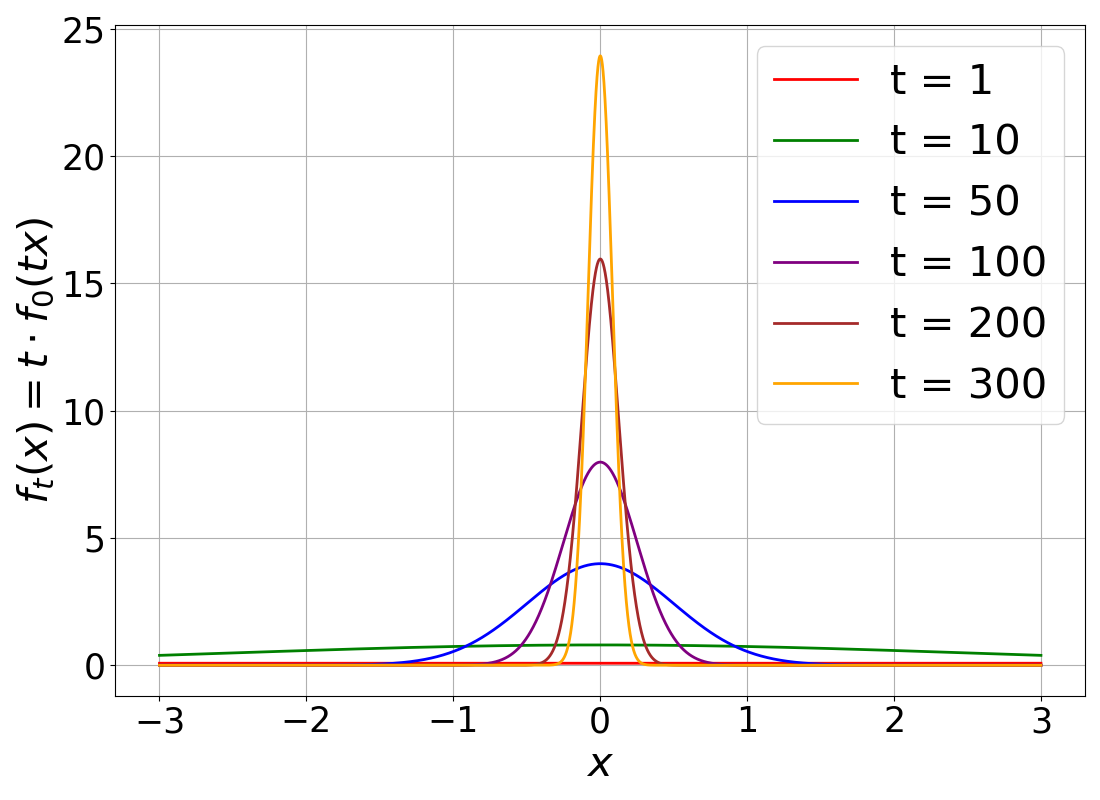
\includegraphics[width = 0.4\linewidth]{pictures/fig1_Normal.png}
            \includegraphics[width = 0.4\linewidth]{pictures/fig1_Uniform.png}
            
            \caption{Пример стремления к $\delta(x)$. $\mathcal{N}(0, 5^2)$ (слева), $\mathcal{U}[-2.5, 2.5]$ (справа).}
            \label{example1_fig}
        \end{figure}

    \subsection{Анализ достаточных условий существования обратной связи}

            В этом разделе исследуется Предположение 1, сформулированное в \cite{khritankov2021hidden}, которое гласит, что в системе \eqref{system} существует петля положительной обратной связи, если оператор $\text{D}_t$ является сжимающим в метрическом пространстве предсказаний модели. Это предположение не было доказано в оригинальной статье, однако в данной работе приводятся результаты, доказывающие ее правильность. Приведем следствие из Теоремы~\ref{delta}, которое оценивает стремление моментов случайных величин невязок модели $h$ к нулю. 
    
            \begin{lemma}[Лемма 1 из \cite{veprikov2024mathematical}] \label{moments}
            Если система \eqref{system} с $n=1$ удовлетворяет условиям Теоремы~\ref{delta} и $\psi_t$ расходятся к бесконечности, тогда все четные моменты случайной величины невязок 
            $y - h(X)$ (если они существуют) убывают со скоростью как минимум $\psi_t^{-2k}$, то есть $\nu_{2k}^t \leq \psi_t^{-2k} \nu_{2k}^0$, где $\nu_{2k}^t$ -- это $2k$-тый момент $y - h(X)$ на шаге $t$.
    
            Если оператор эволюции системы \eqref{system} удовлетворяет \eqref{cool_D}, тогда все (не только четные) моменты случайной величины
            $y - h(X)$ (если они существуют) убывают со скоростью $\psi_t^{-k}$.
    
            Если существует $q \in [1; +\infty]$ такой, что $\{\nu_k^0\}_{k=1}^{+\infty} \in l_q$ и оператор эволюции системы \eqref{system} удовлетворяет \eqref{cool_D}, тогда $\{\nu_k^t\}_{k=1}^{+\infty} \in l_1$ и $\{\nu_k^t\}_{k=1}^{+\infty} \underset{t \to \infty}{\overset{l_1}{\longrightarrow}} 0$.
        \end{lemma}

        \begin{proof}
            Для начала докажем первую часть Леммы~\ref{moments}. По определению $k$-того момента получаем:
            \begin{equation*}
                \nu_{2k}^t = \int\limits_{-\infty}^{+\infty} x^{2k} f_t(x) dx \leq \int\limits_{-\infty}^{+\infty} x^{2k} \psi_t g(\psi_t x) dx.
            \end{equation*}
            
           Это неравенство выполнено, так как $x^{2k} \geq 0$. Сделаем замену переменных: $y = \psi_t \cdot x$, тогда получим:
            \begin{equation*}
                \nu_{2k}^t \leq \int\limits_{-\infty}^{+\infty} \dfrac{y^{2k}}{\psi_t^{2k}} g(y) dy = \psi_t^{-2k} \nu_{2k}^0.
            \end{equation*}
            
            Первая часть Леммы~\ref{moments} доказана, рассмотрим вторую. Если оператор эволюции системы \eqref{system} удовлетворяет \eqref{cool_D}, тогда:
            \begin{equation*}
                \nu_{k}^t = \int\limits_{-\infty}^{+\infty} \dfrac{y^k}{\psi_t^k} g(y) dy = \psi_t^{-k} \nu_{k}^0.
            \end{equation*}
            
            Вторая часть Леммы~\ref{moments} доказана, рассмотрим третью.
            \begin{equation*}
                \|\{\nu_k^t\}_{k=1}^{+\infty}\|_1 = \|\{\psi_t^{-k} \nu_k^0\}_{k=1}^{+\infty}\|_1 \leq \|\{\psi_t^{-k}\}_{k=1}^{+\infty}\|_p \cdot \|\{\nu_k^0\}_{k=1}^{+\infty}\|_q.
            \end{equation*}
            
            Второй шаг следует из неравенства Гёльдера.
            Посчитаем $\|\{\psi_t^{-k}\}_{k=1}^{+\infty}\|_p$ для $p \in [1; +\infty)$:
            \begin{equation*}
                \|\{\psi_t^{-k}\}_{k=1}^{+\infty}\|_p^p = \sum\limits_{k=1}^{+\infty}\psi_t^{-kp} = \dfrac{\psi_t^{-p}}{1 - \psi_t^{-p}} = \dfrac{1}{\psi_t^p - 1}.
            \end{equation*}
            
            Первое равенство выполнено, если $\psi_t > 1$, второй шаг -- это сумма бесконечно убывающей прогрессии. Затем, получаем:
            \begin{equation*}
                \|\{\psi_t^{-k}\}_{k=1}^{+\infty}\|_p = \left( \dfrac{1}{\psi_t^p - 1} \right)^{1/p} \underset{t \to +\infty}{\longrightarrow} 0 ~~~\forall p \in [1; +\infty).
            \end{equation*}
            
            Если $p = +\infty$:
            \begin{equation*}
                \|\{\psi_t^{-k}\}_{k=1}^{+\infty}\|_{\infty} = \left[ \text{ если } \psi_t > 1 \right] = \psi_t^{-1} \underset{t \to +\infty}{\longrightarrow} 0.
            \end{equation*}
            
            Следовательно: 
            \begin{equation*}
                \|\{\nu_k^t\}_{k=1}^{+\infty}\|_1 \leq \|\{\psi_t^{-k}\}_{k=1}^{+\infty}\|_p \cdot \|\{\nu_k^0\}_{k=1}^{+\infty}\|_q \underset{t \to +\infty}{\longrightarrow} 0.
            \end{equation*}
            
            Так как $\|\{\nu_k^0\}_{k=1}^{+\infty}\|_q < +\infty$ по условию Леммы~\ref{moments}.
        \end{proof}
    
        \paragraph{Обсуждение Леммы~\ref{moments}.} Лемма~\ref{moments} интересна с практической точки зрения, так как вычисления моментов случайных величин гораздо более проще проверить в вычислительном эксперименте, чем условия Теоремы~\ref{delta}. 
    
        Эта лемма также помогает в исследовании Предположения 1 из \citep{khritankov2021hidden}, поскольку четные моменты, такие как дисперсия, можно рассматривать в качестве метрики качества предсказаний регрессионной модели. Следовательно, если существует стремление к дельта-функции, то отображение $\text{D}_t$ является сжимающим в пространстве метрик. Если же последовательность $f_t$ стремится к дельта-функции, то в системе \eqref{system} существует петля положительной обратной связи, то есть Предположение 1 из \cite{khritankov2021hidden} в этом случае верно.
    
        В следующей лемме также делается попытка проанализировать Предположение 1 в нашей постановке задачи \eqref{system}.
    
        \begin{lemma}[Лемма 2 из \cite{veprikov2024mathematical}] \label{ineq_q}
            Рассмотрим функцию
            \begin{equation*}
                f_A(x) = \dfrac{1}{\lambda(A)} \cdot \textbf{1}_{A}(x),
            \end{equation*}
            где $A \subset \mathbb{R}^n$ произвольное измеримое по Лебегу множество ненулевой меры и $\lambda(A) > 0$ -- мера множества $A$.
    
            Тогда для любого $A \subset \mathbb{R}^n$ такого, что $\lambda(A) \in (0; +\infty)$ и для всех $q \in [1; +\infty]$ таких, что $\text{D}_t(f_A) \in L_q(\mathbb{R}^n)$ выполнено следующее неравенство
    
            \begin{equation*}
                \|\text{D}_t\|_q \geq \int\limits_{A} \text{D}_t(f_A)(x)dx.
            \end{equation*}
        \end{lemma}

        \begin{proof}
            Для начала посчитаем $\|f_A\|_p$:
            \begin{equation*}
                \|f_A\|_p = \left( \text{ } \int\limits_{\mathbb{R}^n}\left(\dfrac{1}{\lambda(A)}\right)^p \cdot \textbf{1}_{A}(x) dx \text{ } \right)^{1/p} = \dfrac{1}{\lambda(A)} \cdot (\lambda(A))^{1/p} = (\lambda(A))^{-1 + 1/p}.
            \end{equation*}
            
            То есть, $f_A \in L_p(\mathbb{R}^n)$ для всех $A \subset \mathbb{R}^n : 0 < \lambda(A) < +\infty$ и $1 \leq p \leq +\infty$. 
            Теперь используем неравенство Гёльдера. Для $q$ такого, что $p^{-1} + q^{-1} = 1$ выполнено следующее неравенство:
            \begin{equation*}
                \|f_A\|_p \cdot \|\text{D}_t(f_A)\|_q \geq \|f_A \cdot \text{D}_t(f_A)\|_1.
            \end{equation*}
            
            Используя распространенное неравенство на операторные нормы $\|\text{D}_t(f)\|_q \leq \|\text{D}_t\|_q \cdot \|f\|_q ~\forall f \in L_q(\mathbb{R}^n)$, получаем:
            \begin{equation*}
                \|f_A\|_p \|f_A\|_q \cdot \|\text{D}_t\|_q \geq \|f_A \cdot \text{D}_t(f_A)\|_1.
            \end{equation*}
            
            Так как $\|f_A\|_p \|f_A\|_q = (\lambda(A))^{-1 + 1/p} \cdot (\lambda(A))^{-1 + 1/q} = (\lambda(A))^{-2 + 1/p + 1/q} = (\lambda(A))^{-1}$, получаем:
            \begin{equation*}
                \|\text{D}_t\|_q \geq \lambda(A) \cdot \|f_A \cdot \text{D}_t(f_A)\|_1.
            \end{equation*}
            
            Рассмотрим $\|f_A \cdot \text{D}_t(f_A)\|_1$:
            \begin{equation*}
                \|f_A \cdot \text{D}_t(f_A)\|_1 = \int\limits_{\mathbb{R}^n} \text{D}_t(f_A)(x) \cdot \dfrac{1}{\lambda(A)} \textbf{1}_{A}(x) dx = \dfrac{1}{\lambda(A)} \int\limits_{A} \text{D}_t(f_A)(x)dx.
            \end{equation*}
            
            Итого, получаем нужное неравенство:
            $
                \|\text{D}_t\|_q \geq \int_{A} \text{D}_t(f_A)(x)dx.
            $
        \end{proof}
    
        \paragraph{Обсуждение Леммы~\ref{ineq_q}.} Прежде всего, отметим, что результат Леммы~\ref{ineq_q} никак не зависит от того, является ли $\text{D}_t$ преобразованием на $\textbf{F}$ или нет, он является следствием неравенства Гёльдера.
    
        Если рассматривать постановку задачи из данной работы, то $\text{D}_t$ переводит $\textbf{F}$ в $\textbf{F}$, тогда функция $f_A$ является плотностью векторов, равномерно распределенных на множестве $A$. Следовательно, $\int_{A} \text{D}_t(f_A)(x)dx \leq 1$, то есть из Леммы~\ref{ineq_q} можно заключить, что $\| \cdot \|_q$ норма оператора $\text{D}_t$ больше или равна единице. Но если $\|\text{D}_t\|_q \geq 1$, то $\text{D}_t$ не будет сжимающим отображением в $\|\cdot\|_q$, потому что всегда найдется функция $f \in \textbf{F}$ такая, что $\|\text{D}_t(f)\|_q \geq \|f\|_q$. Это важно, потому что если в системе \eqref{system} существует стремление к нулевому распределению $\zeta(x)$, то отображения $\text{D}_t$ будут сжимающими в любой норме $\| \cdot \|_q$, то есть $\left\|\text{D}_t\right\|_q \leq 1$. 
    
        Лемма~\ref{ineq_q} помогает в исследовании Предположения~1 из предыдущей работы \citep{khritankov2021hidden}. Если отображение $\text{D}_t$ не является сжимающим по $\| \cdot \|_q$ норме, то есть $\left\|\text{D}_t\right\|_q \geq 1$, то оно будет сжимающим в векторном пространстве метрик качества модели регрессии, так как $\| \cdot \|_q$ норма функций увеличивается по мере их стремления к дельта-функции.
    
    \subsection{Критерий автономности}
    
        Автономность -- важное свойство любой динамической системы. Такие системы не зависят от начального времени $t_0$, с которого началось наблюдение за ней. Также в Теореме~\ref{delta} данной статьи рассматривается стремление временного шага $t$ к бесконечности, но на практике могут быть рассмотрены только конечные $t$. Однако, если система автономна, можно изучать её на ограниченном интервале и понять поведение системы при бесконечном $t$.
    
        Из Теоремы~\ref{delta} следует, что существует специальный вид отображений \eqref{cool_D}, которые ограничивают функции плотности распределения данных системы сверху, и именно отображения этого типа будут рассмотрены в этом разделе. Для таких отображений можно вывести критерий автономности системы \eqref{system}.
    
        \begin{theorem}[Теорема 4 из \cite{veprikov2024mathematical}] \label{semigroup}
            Если операторы эволюции $\text{D}_t$ динамической системы \eqref{system} имеют вид \eqref{cool_D}, тогда система \eqref{system} автономна тогда и только когда, когда
            \begin{equation} \label{cond_semigroup}
                \psi_{\tau + \kappa} = \psi_{\tau} \cdot \psi_{\kappa} ~\forall \tau, \kappa \in \mathbb{N}.
            \end{equation}
        \end{theorem}

        \begin{proof}
            Для начала посчитаем:
            \begin{equation*}
            (\text{D}_{\overline{1, \tau}} \circ \text{D}_{\overline{1, \kappa}})(f)(x) = \text{D}_{\overline{1, \tau}}(\psi_{\kappa}^n \cdot f(\psi_{\kappa} \cdot x)) = \psi_{\tau}^n\psi_{\kappa}^n \cdot f(\psi_{\tau}\psi_{\kappa} \cdot x),
            \end{equation*}

            С другой стороны,
            $
                \text{D}_{\overline{1, \tau + \kappa}}(f)(x) = \psi_{\tau + \kappa}^n \cdot f(\psi_{\tau + \kappa} \cdot x).
            $
            То есть система \eqref{system} автономна тогда и только когда $\psi_{\tau + \kappa} = \psi_{\tau} \cdot \psi_{\kappa}$ для всех $ \tau, \kappa \in \mathbb{N}$.
        \end{proof}
    
        \paragraph{Обсуждение Теоремы~\ref{semigroup}.} Критерий из Теоремы \ref{semigroup} легко проверяем на практике, так как условие \eqref{cond_semigroup} означает, что последовательность $\psi_t$ является степенной последовательностью, то есть $\psi_t = a^t$ для некоторого $a > 0$. 
    
        Пример отображения вида \eqref{cool_D} приведен в Разделе~\ref{sec:experiments} под названием \emph{Обновление выборки}.
    
        Автономность системы позволяет экспериментально определить форму графика $\psi_t$, который должен быть похож на степенную функцию. В вычислительном эксперименте демонстрируется, как Теорема~\ref{semigroup} может быть проверена на практике.
    
    \subsection{Сохранение предельного множества при преобразовании признаков}

        В данном разделе анализируется оператор $G$, осуществляющий преобразование пространства признаков $X$ и целевой переменной $y$ для модели машинного обучения в задаче обучения с учителем. Целью данного раздела является нахождение достаточных условий, при которых предельное распределение для системы невязок, полученное с помощью Теоремы \ref{delta}, сохраняется при преобразовании $(X, y) \to G(X, y)$. 

        При переходе от данных к невязкам модели, даже при использовании гладких и биективных $G$, не очевидно, что предельное распределение сохранится, приведем пример. Допустим, что $G$ -- это поворот на $45$ градусов против часовой стрелки и пусть данные имеют вид $y = x + \varepsilon_t$, где  $\varepsilon_t \sim \mathcal{N}(0; \sigma_t^2)$ -- случайный шум на шаге $t$. Тогда при решении задачи регрессии с линейной моделью, невязки будут распределены как $\varepsilon_t$, и если $\sigma_t \to 0$, то функции плотности невязки на шаге $t$ стремятся к дельта-функции. Однако, если повернуть данные, $y$ перестает зависеть от $x$, и в таком случае предельное распределение изменится, так как невязки моделей будут большими. 

        Приведем другой пример, когда происходит обратная ситуация. По теореме Цыбенко \cite{cybenko1989approximation} любую непрерывную функцию можно с любой наперед заданной точностью аппроксимировать с помощью нейронной сети с одним скрытым слоем. Таким образом, преобразование $G$ может служить переходом от входных данных $X$ к их представлению на скрытом слое. В таком случае, до преобразования невязки модели могли быть большими, однако после применения $G$ точность модели увеличивается и невязки начинают стремиться к дельта функции. Соответственно, нужно исследовать, каким образом $G$ влияет на результат работы модели машинного обучения.

        \begin{lemma} \label{loss}
            Пусть в системе \eqref{system} для невязок задачи обучения с учителем $L(y, h, X)$ -- функция потерь модели $h$, а $(X_t, y_t)$ -- выборка на шаге $t$, $(X_t', y_t') = G(X_t, y_t)$ – выборка после применения оператора $G$. 
            
	        Тогда если существует $T \in \mathbb{N}$ такой, что для всех $t \geq T$ выполнено $L(y_t, h_t, X_t) \geq L(y_t', h_t', X_t')$ и функции плотности невязок $y_t - h_t(X_t)$ стремились к дельта-функции $\delta(x)$, то функции плотности $y_t' - h_t'(X_t')$ также стремятся к дельта-функции. 
         
	        Если же существует $T \in \mathbb{N}$ такой, что для всех $t \geq T$ выполнено $L(y_t, h_t, X_t) \leq L(y_t', h_t', X_t')$ и функции плотности невязок $y_t - h_t(X_t)$ стремились к нулевому распределению $\zeta(x)$, то функции плотности $y_t' - h_t'(X_t')$ также стремятся к нулевому распределению. 
        \end{lemma}

        \begin{proof}
            Пусть функции плотности невязок $f_t(x)$ стремились к дельта функции $\delta(x)$ слабо. Тогда если преобразование $G$, начиная с какого-то $T$, будет уменьшать функцию потерь для всех $t \geq T$, то будет выполнено следующее неравенство: 
            $L(y_t, h_t, X_t) \geq L(y_t', h_t', X_t')$. Но так как $L(y_t, h_t, X_t) \to 0$, так как изначальные функции плотности невязок $f_t(x)$ стремились к дельта-функции $\delta(x)$, то  $L(y_t', h_t', X_t') 0$. Соответственно, новые функции плотности невязок также стремятся к дельта-функции. Аналогично доказывается вторая часть Леммы~\ref{loss}: если если преобразование $G$ начиная с какого-то $T$ будет увеличивать функцию потерь для всех $t \geq T$, то будет выполнено следующее неравенство: $L(y_t, h_t, X_t) \leq L(y_t', h_t', X_t')$. Но так как $L(y_t, h_t, X_t) \to \infty$, так как изначальные функции плотности невязок $f_t(x)$ стремились к нулевому распределению $\zeta(x)$, то  $L(y_t', h_t', X_t') \to \infty$ . Соответственно, новые функции плотности невязок также стремятся к нулевому распределению.
        \end{proof}

        \paragraph{Обсуждение Леммы~\ref{loss}.} Поскольку аналитическая проверка неравенств для функций потерь, представленных в Лемме~\ref{loss}, представляет собой сложную задачу, предлагается экспериментальный подход к проверке выполнимости этих неравенств для преобразования $G$. Согласно работе \cite{domingos2000unified}, квадратичная (MSE) и другие функции потерь, часто применяемые в задаче регрессии, могут быть разложены на составляющие смещения: $\text{Bias}(y, h, X) = \mathbb{E}\left[ y(X) - h(X)\right]$, разброса: $\text{Var}(y, h, X) = \mathbb{E}\left[ \left(h(X) - \mathbb{E}\left[ h(X) \right] \right)^2\right]$ и неустранимого шума в данных $\sigma^2$:
        $L(y, h, X) = \text{Bias}(y, h, X)^2 + \text{Var}(y, h, X) + \sigma^2.$
        Разброс и смещение измеримы экспериментально в ходе обучения модели.

        \begin{lemma} \label{bvd}
            Пусть существует $T \in \mathbb{N}$ такой, что для всех $t \geq T$ преобразование $G$ уменьшает сумму смещения и разброса на шаге $t$, тогда $L(y_t, h_t, X_t) \geq L(y_t', h_t', X_t')$ для всех $t \geq T$.
            
	        Если же для всех $t \geq T$ преобразование $G$ увеличивает сумму смещения и разброса на шаге $t$, тогда выполнено обратное неравенство: $L(y_t, h_t, X_t) \leq L(y_t', h_t', X_t')$ для всех $t \geq T$.
        \end{lemma}

        \begin{proof}
            Так как согласно \cite{domingos2000unified} любую функцию ошибки $L$ можно разложить на составляющие смещения и разброса, то при уменьшении (или увеличении) их суммы будет уменьшаться (или увеличиваться) и функция ошибки.
        \end{proof}

        \paragraph{Обсуждение Леммы~\ref{bvd}.} Примерами преобразований $G$, которые удовлетворяют первой части Леммы~\ref{bvd}, могут служить добавление значимых признаков, использование линейных преобразований в пространство большей размерности и так далее. Для некоторых преобразований не понятно, уменьшиться ли значение функции потерь, например при нормировке признаков, однако эвристически можно предполагать, что популярные преобразования не увеличивают значение функции потерь.



        

        


        

    
    

        